\section{Results}
\label{sec:results}

\subsection{The shape and growth of the field}

Quarterly output in the coded corpus rose from \firstQn{} papers in \firstQ{} to \peakQn{} in
\peakQ{} --- roughly \growthFactor{}-fold in nine quarters (Figure~\ref{fig:growth}). The
partial quarter \partialQ{} already contains \partialQn{} papers from July alone. Growth of
this kind means any narrative survey is stale on publication, which is part of why we release
the pipeline rather than only the findings.

The corpus divides into \nSystem{} system papers, \nBenchmark{} benchmarks, \nFramework{}
frameworks, \nPosition{} position papers, \nCaseStudy{} case studies, and \nSurvey{} surveys.
Its centre of gravity is computational: the largest domain is machine learning research itself,
with materials, biomedicine, and physics forming a substantial experimental minority.

\begin{figure}[t]
\centering
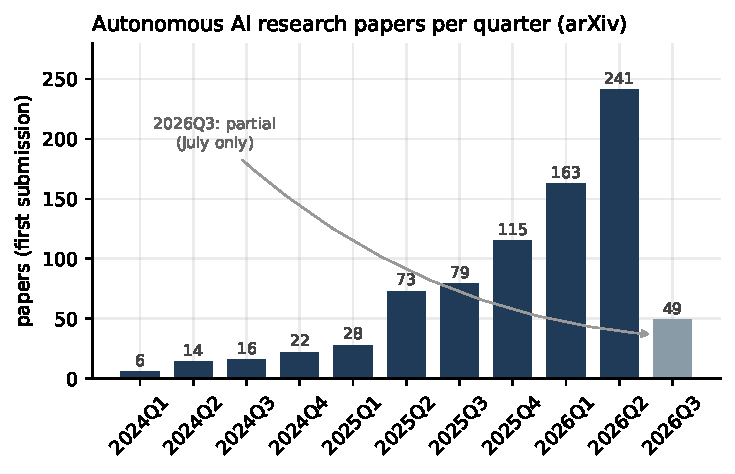
\includegraphics[width=0.85\textwidth]{../figures/fig1-growth.pdf}
\caption{Papers on autonomous AI research systems per quarter of first arXiv submission
(coded corpus, $n=\nCorpus{}$). The final bar covers July 2026 only.}
\label{fig:growth}
\end{figure}

\subsection{What these systems do, and how autonomously}

Figure~\ref{fig:stages} shows lifecycle coverage and demonstrated autonomy. Literature
synthesis is the most commonly automated stage, followed by analysis and ideation; peer
review is the least. Experiment execution appears in a substantial minority, reflecting the
self-driving-laboratory subliterature.

Autonomy is more revealing. Of the \nSystemsCoded{} papers presenting a system or case study,
\nClosedLoop{} demonstrate a closed multi-stage loop with humans monitoring rather than gating,
and only \nFullAuto{} claim full autonomy from question to manuscript. The modal system
automates a single stage end to end. The field's rhetoric is dominated by end-to-end
autonomy; its demonstrated practice is not.

\begin{figure}[t]
\centering
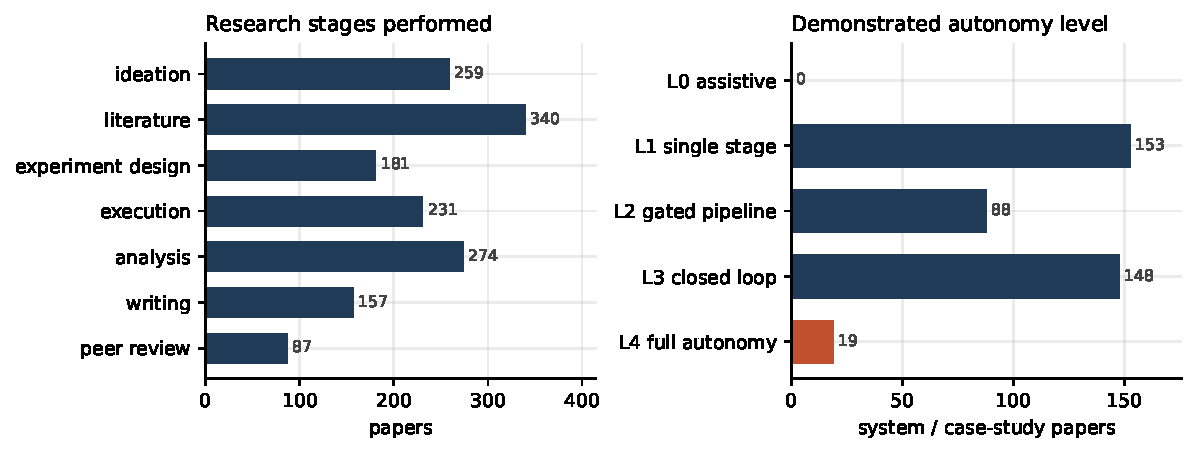
\includegraphics[width=\textwidth]{../figures/fig2-stages-autonomy.pdf}
\caption{Left: research-lifecycle stages substantively performed (multi-select). Right:
highest autonomy level actually demonstrated, among papers presenting a system or case study.}
\label{fig:stages}
\end{figure}

\subsection{The evidentiary picture}
\label{sec:evidence}

Figure~\ref{fig:verification} is the central result. By the conventions of machine-learning
publication the corpus evaluates itself thoroughly: benchmark metrics are near-universal.
But the evaluations that would let a reader check a specific claim are rare.

\begin{itemize}\itemsep2pt
\item \pctHeldOut{} of papers re-test a selected result outside the loop that produced it.
\item \pctRealWorld{} report any external validation --- wet-lab confirmation, deployment,
reproduction of established results, or peer-review acceptance of generated work.
\item \pctHumanExpert{} involve domain experts in assessing outputs, while \pctLLMJudge{} use
LLM judges; \pctNoEval{} report no empirical evaluation at all.
\item \pctAuditNone{} --- \nAuditNone{} papers --- provide \emph{no} auditability mechanism:
no inspectable traces, no claim-to-evidence provenance, no reproduction artifacts, no
machine-checkable verification, no calibration reporting. Formal verification appears in
\nFormalVerif{} papers.
\end{itemize}

\begin{figure}[t]
\centering
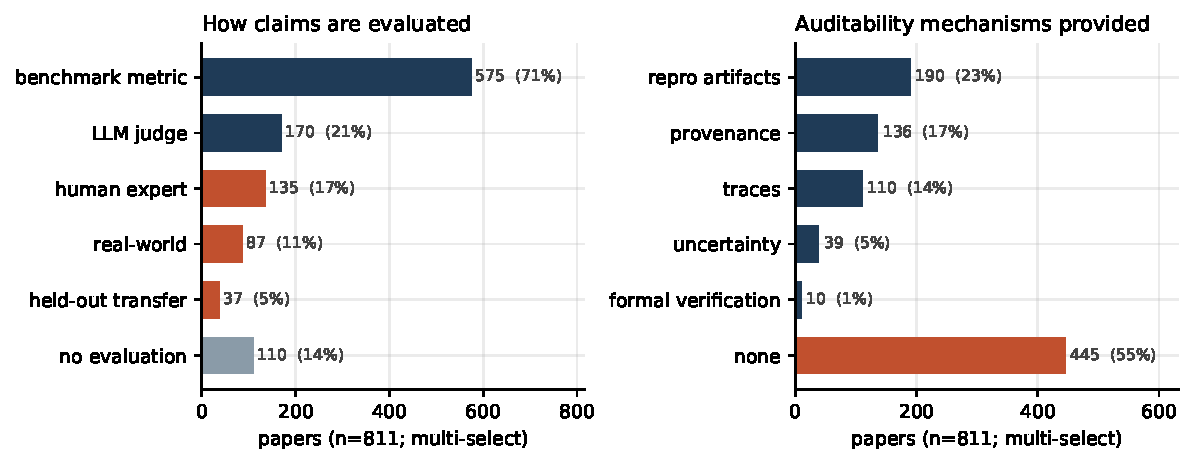
\includegraphics[width=\textwidth]{../figures/fig3-verification.pdf}
\caption{Evaluation methods (left) and auditability mechanisms (right) across the corpus
($n=\nCorpus{}$, multi-select). Highlighted bars mark evaluations that test a claim outside
the loop that produced it, and the share of papers offering no auditability mechanism.}
\label{fig:verification}
\end{figure}

\subsection{Claims outrun evidence exactly where it matters}

The prespecified operationalisation of the auditability gap --- a strong claim paired with
evaluation limited to LLM judging or nothing, and no released code --- flags \nWeakStrong{}
papers (\pctWeakStrong{}). We report that figure as specified, but it is insensitive: it
treats any benchmark metric as adequate verification, which is precisely the assumption in
question.

Conditioning on claim strength is more informative (Figure~\ref{fig:gap}). The corpus makes
\nMethodClaim{} method claims, \nCapability{} capability claims, \nConceptual{} conceptual
claims, and \nDiscovery{} discovery claims --- assertions that the AI produced new knowledge
about the world. Discovery claims are the ones a reader most needs to be able to check, and
they are among the least checkable: \pctDiscNoAudit{} of them provide no auditability
mechanism, and only \pctDiscRealWorld{} report external validation. Of the discovery papers
we verified from full text, \pctDiscRepo{} link a code repository.

\begin{figure}[t]
\centering
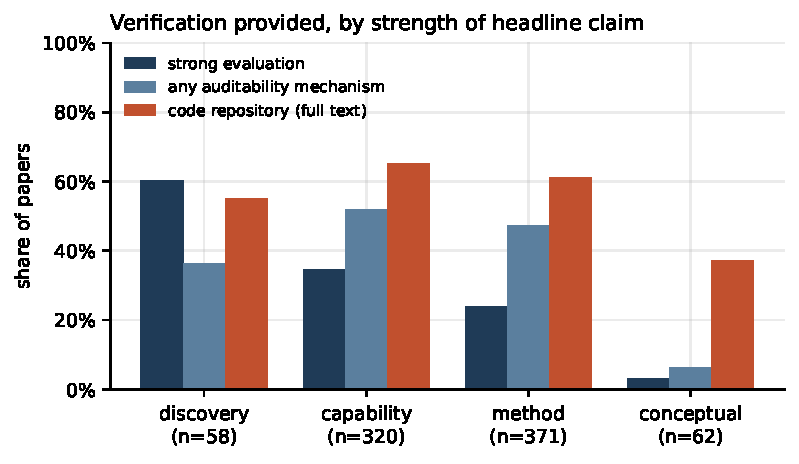
\includegraphics[width=0.85\textwidth]{../figures/fig4-claim-vs-evidence.pdf}
\caption{Share of papers providing strong evaluation, any auditability mechanism, and a
full-text-verified code repository, by strength of headline claim.}
\label{fig:gap}
\end{figure}

\subsection{The missing human}

The dimension we did not expect to be the starkest is the role of humans.
\pctHumanUnspec{} of the corpus --- \nHumanUnspec{} papers --- either claims no human
involvement or leaves the human role unstated. Papers that name a specific human function
(gatekeeper, evaluator, or co-performer) are a minority.

This matters for interpreting every other number here. When a paper reports that a system
autonomously produced a result, the reader usually cannot tell whether a human selected the
task, chose the baseline, restarted a failed run, discarded a bad trajectory, or edited the
output. In our own project --- documented in Section~\ref{sec:reflexive} --- human
intervention changed the corpus by 183 papers, and a reader who was told only that ``an AI
conducted a systematic review'' would have no way to know that. We suspect the same is true
across much of this literature, and note that it is cheap to fix: a sentence stating what
humans did costs nothing and is currently absent from roughly seven papers in ten.

\subsection{Artifact release, measured rather than inferred}

Full-text verification of \nArtChecked{} papers finds repository links in \pctRepo{}, against
\pctRepoAbstract{} inferable from abstracts (Section~\ref{sec:artifacts}). Two points follow.
First, the field releases code more often than abstract-level reading suggests, and we correct
our own earlier estimate accordingly. Second, systematic reviews that code artifact release
from abstracts --- a common practice --- should expect a bias of this magnitude.
